\subsection{Overview of systematic}
\label{lab:Systematic_overvies}

Sources of systematic effects can be considered as nominal analysis in ATLAS, but following items are canceled out by taking the double ratio. 

\begin{itemize}
\item[a] Theory related items, i.e. cross section of all SM processes, QCD scale uncertainty, any kinematic mismodling including higher order calculation in the Matrix element or parton shawer, variation of parton distribution functions. 
\item[b] Most of experimental items, i.e., object reconstruction and identification efficiencies, total luminosity, normalization effects.
\item[c] year by year normnalization effect, i.e., LUCID luminosity measurement variation.
\item[d] mis-measurement on Z counting or LUCID luminosity. 
\item[e] Time dependent effects, i.e.  $\left< \mu \right>$ effect.

\end{itemize}

Only time dependent effects remained as systematic uncertainty, therefore items ``a'' and ``b'' are not the source of systematic on the LIV search.

Concerning to item ``c'', there are variation in the LUCID luminosity measurement, which effect are corrected by van-deer-mir scan. If we sum up all years (2015 to 2018) into one double ratio, this would introduce additional systematic effect, but as we discussed in Section~\ref{lab:DataScrambling}, we build the double ratio each year separately and combine in the final fit. Therefore, this effect is not necessary to take into account.

Nevertheless, item ``d'', mis-measurement on the input of the double ratio could introduce the systematic effect. In order to exclude mis-measurement, LBs have large deviation, i.e. integrated luminosity would be 0 in one of input (either LUCID, electron channel or muon channel of Z counting luminosity) are excluded from the input LB as additional data quality requirement. 


The item ``e'' is the systematic source we need to take into account. Actully, the Z counting luminosity measurement does takes into account variation of the trigger and the identification  efficiencies for each LB. 
Therefore, even efficiency variation (in item ``c'') is NOT the dominat source of systematic effect for this analysis.  The statistics uncertainty of 
the efficiency correction in each LB is taken into account and propagaed to the error bar of each phase bin of the double ratio. 

There is a correction factor as function of  $\left< \mu \right>$ in the Z counting measurement, which is FMC correction factor. 
The $\left< \mu \right>$ dependence of $F^\text{MC}_{Z\rightarrow \ell^+\ell^-}$ is fitted with a second-order polynomial per decay channel 
and per data-taking period, and the fit results are shown in Figure~\ref{fig:Zcount:MC correction factors}.

The $Z\rightarrow e^+e^-$ correction factor is >10\% below unity for all $\left< \mu \right>$, implying that there are additional efficiency 
effects beyond those captured in the tag-and-probe procedure. The variation between $\left< \mu \right>=20$ and $\left< \mu \right>=50$ is 
around 2\%, suggesting that pileup-dependent effects are mild.

\begin{figure}[!htb]
        \centering
        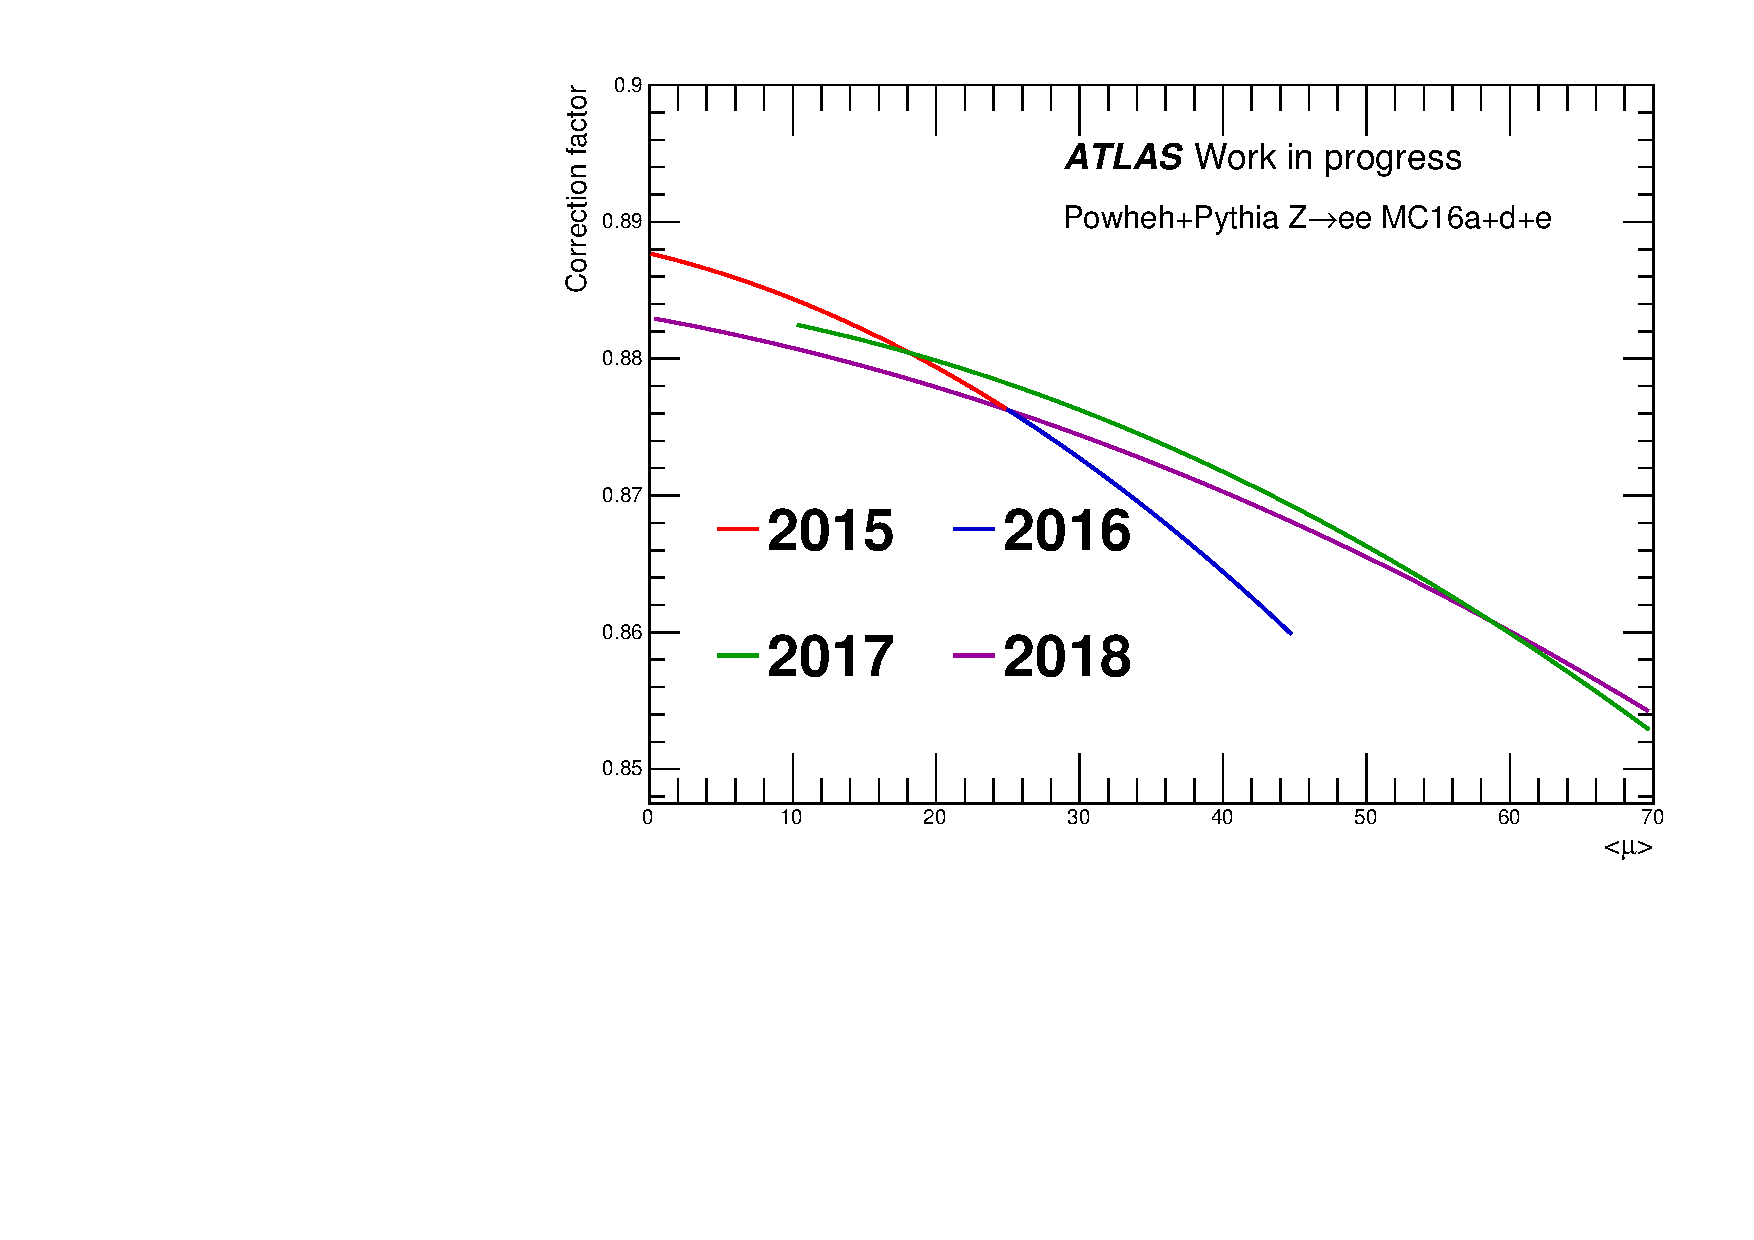
\includegraphics[width=0.6\textwidth]{figs/Zcount/YearlyFMC_ele.pdf}
        \caption{$Z\rightarrow e^+e^-$ correction factors used for each year of data produced using the dedicated Monte Carlo campaigns. The 
          lines show second-order polynomial fits to the correction factor for the corresponding $\left< \mu \right>$ range per year.}
        \label{fig:Zcount:MC correction factors}
\end{figure}

The fits of $F^\text{MC}_{Z\rightarrow \ell^+\ell^-}$, as shown in Figure~\ref{fig:Zcount:MC correction factors}, 
are used in the determination of the Z-counting based luminosity per data-taking period and as a function of the 
pileup parameter $\left< \mu \right>$. The statistical uncertainties of the fits are small and are neglected.

The size of systematic on the FMC corrction is estimated by shifting $\left< \mu \right>$ by $\pm 1$ to apply correction. 
This is done by the TOY study described in Section.~\label{lab:ToyStudy}. Figure~\ref{fig:FMC_variation} shows the effect in the double ratio in a Toy experiment. Result with 1000 Toy experiments are summarized in Figure~\ref{fig:FMC_variation_summary}. We observed this effect is small with respect to statistical uncertainty.

%%%%%%%%%%%%%%%%%%%%%%%%%%%%%%%%%%%%%%%%%%%%%%%%%%%%%%
%%%%%%%%%%%%%%%%%%%%%%%%%%%%%%%%%%%%%%%%%%%%%%%%%%%%%%
%%%%%%%%%%%%%%%%%%%%%%%%%%%%%%%%%%%%%%%%%%%%%%%%%%%%%%
%% \subsection{Shift $<\mu>$ by 1}

\begin{figure}[bt]
\centering
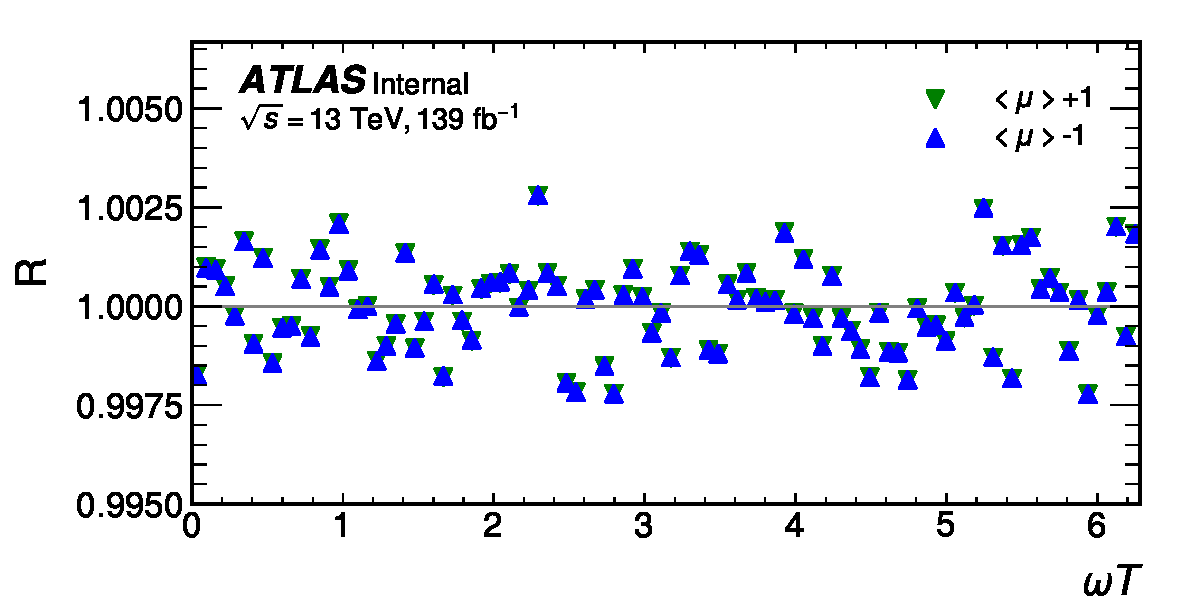
\includegraphics[width=0.95\textwidth]{figs/FMC_sys/compare_input_toy_datasets_mu_shifts} \\
\caption{ Comparison of the toy dataset with average pileup $<\mu>$ increased and decreased by 1. The toy dataset corresponds to four years of Run 2 luminosity is used. The X-axis is the sidereal phase, $\omega T$.
}
\label{fig:FMC_variation}
\end{figure}


\begin{figure}[bt]
\centering
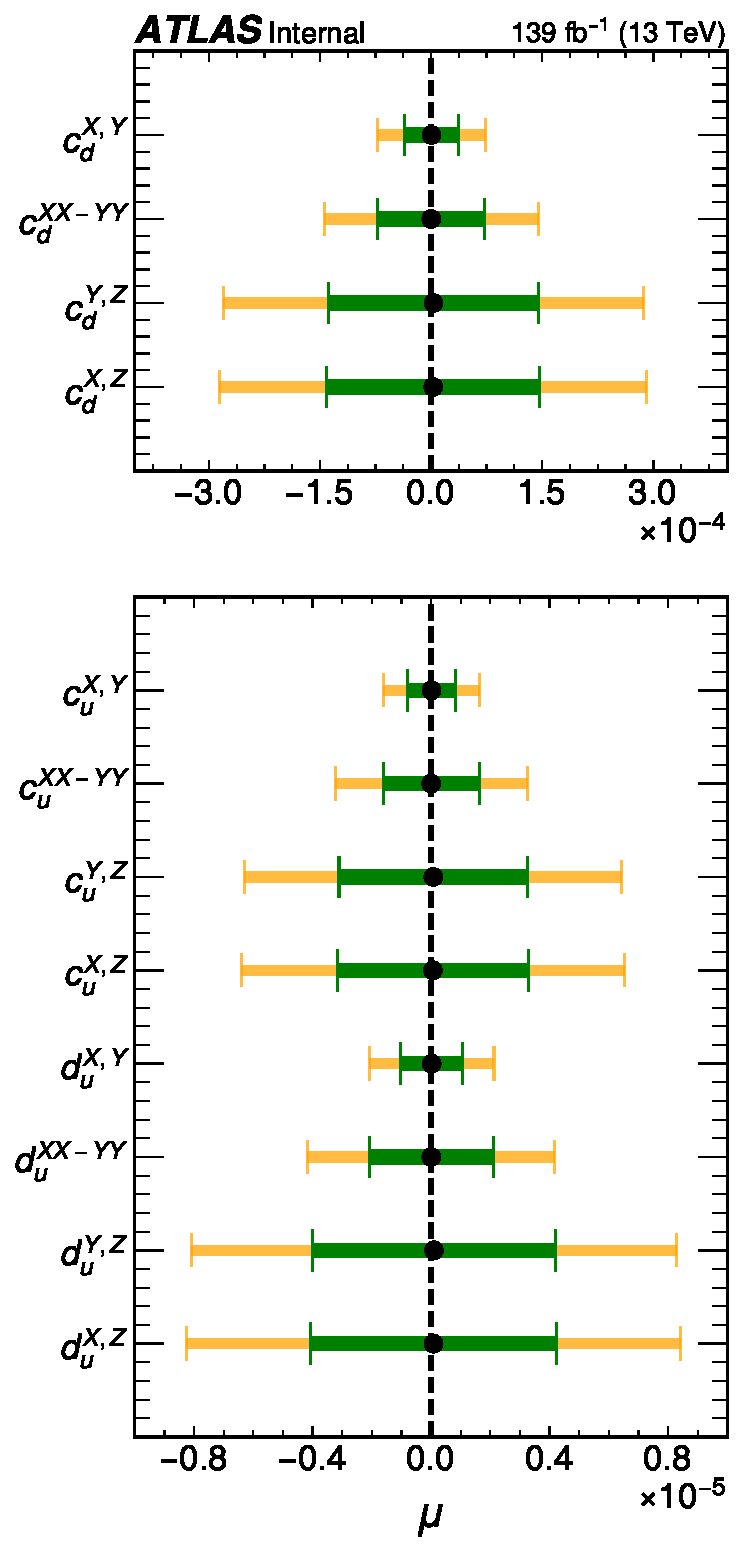
\includegraphics[width=0.4\textwidth]{figs/FMC_sys/SigFit_summary_AllSamples_muShift_p1} 
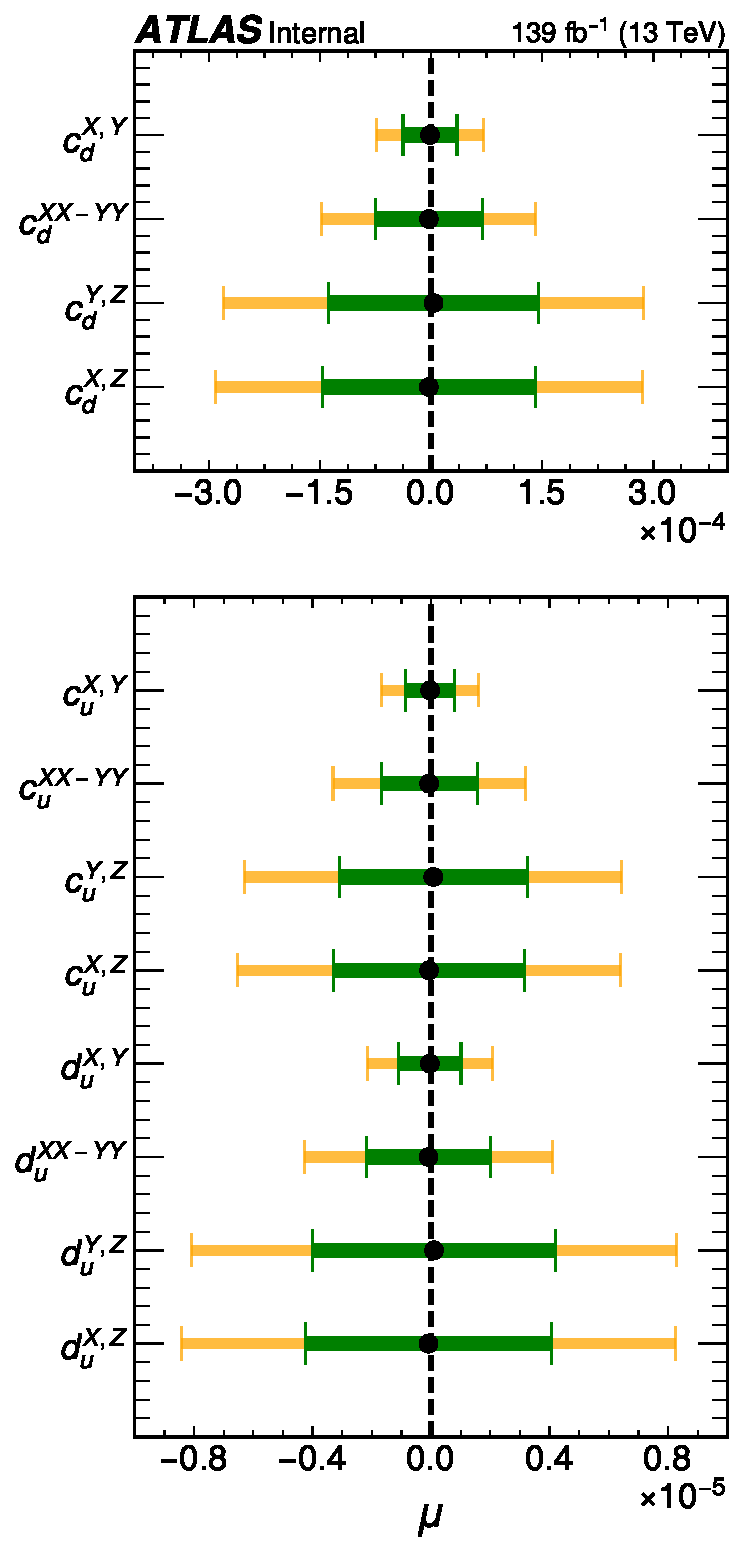
\includegraphics[width=0.4\textwidth]{figs/FMC_sys/SigFit_summary_AllSamples_muShift_m1} 
\caption{ Comparison of the fit results with average pileup $<\mu>$ increased and decreased by 1; left (+1) and right (-1). Results are obtained from 1000 toy datasets corresponding to four years of Run 2 luminosity. The X-axis is the sidereal phase, $\omega T$.
}
\label{fig:FMC_variation_summary}
\end{figure}



